\documentclass[11pt,aspectratio=169]{beamer}

% Theme and colors - Virginia Tech Style
\usetheme{Madrid}
\useinnertheme{circles}

% Virginia Tech Official Colors
\definecolor{vtmaroon}{RGB}{134, 31, 65}      % Chicago Maroon (primary)
\definecolor{vtorange}{RGB}{229, 117, 31}      % Burnt Orange (accent)
\definecolor{vtgray}{RGB}{117, 120, 123}       % Limestone Gray

% Apply VT colors to beamer elements
\setbeamercolor{structure}{fg=vtmaroon}
\setbeamercolor{frametitle}{bg=vtmaroon, fg=white}
\setbeamercolor{palette primary}{bg=vtmaroon, fg=white}
\setbeamercolor{palette secondary}{bg=vtorange, fg=white}
\setbeamercolor{palette tertiary}{bg=vtgray, fg=white}
\setbeamercolor{title}{fg=vtmaroon}
\setbeamercolor{subtitle}{fg=vtgray}
\setbeamercolor{author}{fg=vtmaroon}
\setbeamercolor{institute}{fg=vtgray}
\setbeamercolor{item}{fg=vtorange}
\setbeamercolor{subitem}{fg=vtmaroon}
\setbeamercolor{block title}{bg=vtmaroon, fg=white}
\setbeamercolor{block body}{bg=vtmaroon!10}
\setbeamercolor{block title example}{bg=vtorange, fg=white}
\setbeamercolor{block body example}{bg=vtorange!10}

% Packages
\usepackage{graphicx}
\usepackage{booktabs}
\usepackage{tikz}
\usepackage{amsmath}
\usepackage{palatino}  % VT recommended font
\usetikzlibrary{arrows.meta, positioning, shapes.geometric}

% Remove navigation symbols
\setbeamertemplate{navigation symbols}{}

% Add slide numbers with VT style
\setbeamertemplate{footline}[frame number]

% Title info
\title{Construction.AI}
\subtitle{Knowledge-Graph + Agentic System for\\Material Takeoff, Cut Optimization, and Build Instructions}
\author{Jason Cusati}
\institute{Virginia Tech}
\date{January 2026}

\begin{document}

% =============================================================================
% TITLE SLIDE
% =============================================================================
\begin{frame}
\titlepage
\end{frame}

% =============================================================================
% AGENDA
% =============================================================================
\begin{frame}{Agenda}
\tableofcontents
\end{frame}

% =============================================================================
% SECTION 1: PROBLEM
% =============================================================================
\section{The Problem}

\begin{frame}{}
\centering
\vspace{2em}
{\Huge \textbf{50--80\%}}

\vspace{1em}
{\large of estimator time spent on takeoffs}

\vspace{3em}
{\Huge \textbf{15--20\%}}

\vspace{1em}
{\large lumber waste}

\vspace{3em}
\textit{``0\% productivity growth over 20 years''}

\vspace{0.5em}
\small -- McKinsey
\end{frame}

\begin{frame}{}
\centering
\vspace{2em}
{\Large Plans}

\vspace{1em}
\Huge $\downarrow$

\vspace{1em}
{\Large \textcolor{vtorange}{\textbf{?}}}

\vspace{1em}
\Huge $\downarrow$

\vspace{1em}
{\Large BOM · Cuts · Instructions}

\vspace{2em}
{\large \textit{automatically, accurately, auditably}}
\end{frame}

% =============================================================================
% SECTION 2: SOLUTION
% =============================================================================
\section{Our Solution}

\begin{frame}{Construction.AI: KG-Centered Architecture}
\centering
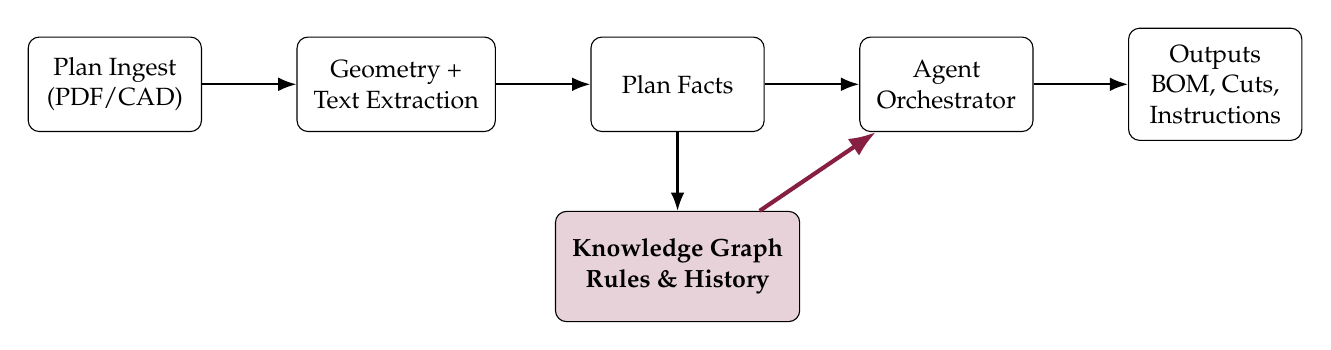
\begin{tikzpicture}[
  node distance=8mm and 12mm,
  box/.style={draw, rounded corners, align=center, inner sep=6pt, font=\small, minimum width=22mm, minimum height=12mm},
  kgbox/.style={draw, rounded corners, align=center, inner sep=6pt, font=\small\bfseries, minimum width=28mm, minimum height=14mm, fill=vtmaroon!20},
  arrow/.style={-Latex, thick}
]
\node[box] (ingest) {Plan Ingest\\(PDF/CAD)};
\node[box, right=of ingest] (extract) {Geometry +\\Text Extraction};
\node[box, right=of extract] (facts) {Plan Facts};
\node[kgbox, below=10mm of facts] (kg) {Knowledge Graph\\Rules \& History};
\node[box, right=of facts] (agents) {Agent\\Orchestrator};
\node[box, right=of agents] (outputs) {Outputs\\BOM, Cuts,\\Instructions};

\draw[arrow] (ingest) -- (extract);
\draw[arrow] (extract) -- (facts);
\draw[arrow] (facts) -- (agents);
\draw[arrow, vtmaroon, line width=1.5pt] (kg) -- (agents);
\draw[arrow] (facts) -- (kg);
\draw[arrow] (agents) -- (outputs);
\end{tikzpicture}

\vspace{0.5em}
\textbf{Key Insight:} Ground every decision in structured knowledge
\end{frame}

\begin{frame}{}
\centering
\vspace{2em}
{\Huge \textbf{Knowledge Graph}}

\vspace{2em}
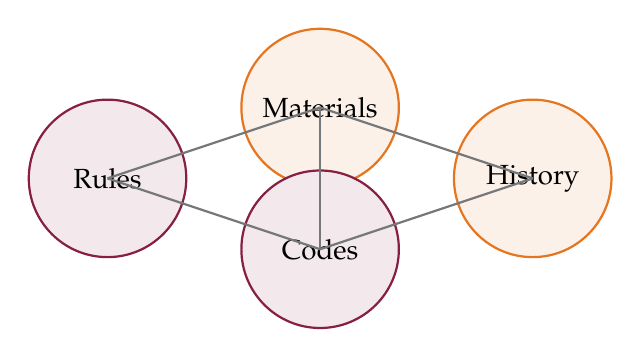
\begin{tikzpicture}[scale=0.9]
\node[circle, draw=vtmaroon, thick, minimum size=2cm, fill=vtmaroon!10] at (0,0) {Rules};
\node[circle, draw=vtorange, thick, minimum size=2cm, fill=vtorange!10] at (3,1) {Materials};
\node[circle, draw=vtmaroon, thick, minimum size=2cm, fill=vtmaroon!10] at (3,-1) {Codes};
\node[circle, draw=vtorange, thick, minimum size=2cm, fill=vtorange!10] at (6,0) {History};
\draw[thick, vtgray] (0,0) -- (3,1);
\draw[thick, vtgray] (0,0) -- (3,-1);
\draw[thick, vtgray] (3,1) -- (6,0);
\draw[thick, vtgray] (3,-1) -- (6,0);
\draw[thick, vtgray] (3,1) -- (3,-1);
\end{tikzpicture}

\vspace{2em}
{\large Structured · Queryable · Evolving}
\end{frame}

% =============================================================================
% SECTION 3: AGENTS
% =============================================================================
\section{Agentic Workflow}

\begin{frame}{Specialized Agents}
\centering
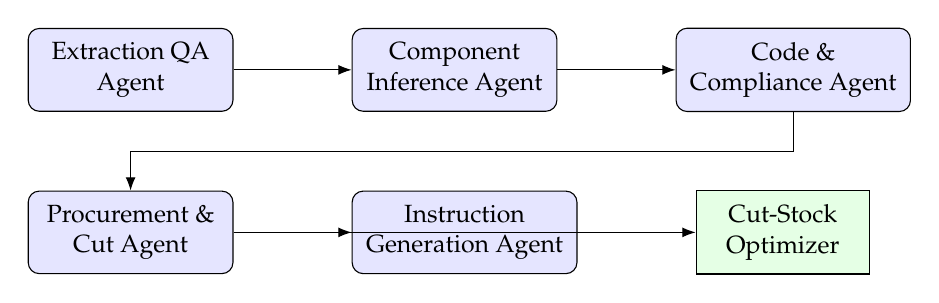
\begin{tikzpicture}[
  node distance=6mm and 15mm,
  agent/.style={draw, rounded corners, align=center, inner sep=5pt, font=\small, fill=blue!10, minimum width=26mm, minimum height=10mm},
  tool/.style={draw, align=center, inner sep=5pt, font=\small, fill=green!10, minimum width=22mm},
  arrow/.style={-Latex}
]
\node[agent] (qa) {Extraction QA\\Agent};
\node[agent, right=of qa] (infer) {Component\\Inference Agent};
\node[agent, right=of infer] (code) {Code \&\\Compliance Agent};
\node[agent, below=10mm of qa] (procure) {Procurement \&\\Cut Agent};
\node[agent, right=of procure] (instruct) {Instruction\\Generation Agent};
\node[tool, right=of instruct] (optimizer) {Cut-Stock\\Optimizer};

\draw[arrow] (qa) -- (infer);
\draw[arrow] (infer) -- (code);
\draw[arrow] (code.south) -- ++(0,-5mm) -| (procure.north);
\draw[arrow] (procure) -- (instruct);
\draw[arrow] (procure) -- (optimizer);
\end{tikzpicture}

\vspace{0.5em}
\textbf{Agents reason; Tools optimize}
\end{frame}

\begin{frame}{}
\centering
\vspace{1em}
{\Large \textbf{5 Specialized Agents}}

\vspace{2em}
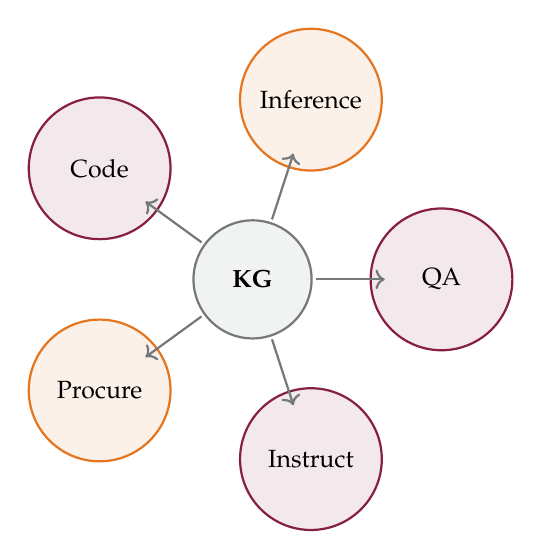
\begin{tikzpicture}[scale=0.8]
\foreach \i/\name/\color in {0/QA/vtmaroon, 72/Inference/vtorange, 144/Code/vtmaroon, 216/Procure/vtorange, 288/Instruct/vtmaroon} {
  \node[circle, draw=\color, thick, minimum size=1.8cm, fill=\color!10, font=\small] at (\i:3cm) {\name};
}
\node[circle, draw=vtgray, thick, minimum size=1.5cm, fill=vtgray!10, font=\small\bfseries] at (0,0) {KG};
\foreach \i in {0,72,144,216,288} {
  \draw[thick, vtgray, ->] (\i:1cm) -- (\i:2.1cm);
}
\end{tikzpicture}

\vspace{2em}
{\large All agents read/write to shared Knowledge Graph}
\end{frame}

% =============================================================================
% SECTION 4: TECHNOLOGY
% =============================================================================
\section{Technology Stack}

\begin{frame}{Parsing \& Extraction}
\begin{table}
\centering
\begin{tabular}{ll}
\toprule
\textbf{Format} & \textbf{Technology} \\
\midrule
PDF (vector) & PyMuPDF \\
PDF (raster) & pdf2image + OpenCV \\
DXF/DWG & ezdxf / LibreDWG \\
OCR & EasyOCR \\
Object Detection & YOLOv8 \\
Scale Detection & Gemini Vision API \\
\bottomrule
\end{tabular}
\end{table}

\vspace{0.5em}
\textbf{Already implemented} in current codebase
\end{frame}

\begin{frame}{}
\centering
\vspace{2em}
{\Huge \textbf{15--20\%}}

\vspace{1em}
{\large typical waste}

\vspace{2em}
\Huge $\downarrow$

\vspace{2em}
{\Huge \textcolor{vtorange}{\textbf{<5\%}}}

\vspace{1em}
{\large optimized waste}

\vspace{2em}
\small $\min \sum_{s \in S} c_s \cdot x_s + \lambda \cdot \text{waste}$
\end{frame}

\begin{frame}{Knowledge Graph \& Agents}
\begin{columns}
\column{0.5\textwidth}
\textbf{Graph Stack:}
\begin{itemize}
    \item Neo4j graph database
    \item Cypher query language
    \item Vector embeddings for semantic search
    \item Async Python driver
\end{itemize}

\column{0.5\textwidth}
\textbf{Agent Stack:}
\begin{itemize}
    \item Claude / GPT-4 LLMs
    \item LangChain orchestration
    \item ReAct reasoning patterns
    \item Structured tool calling
\end{itemize}
\end{columns}
\end{frame}

% =============================================================================
% SECTION 5: OUTPUTS
% =============================================================================
\section{Outputs \& Integration}

\begin{frame}{}
\centering
\vspace{2em}
{\LARGE \textbf{Outputs}}

\vspace{2em}
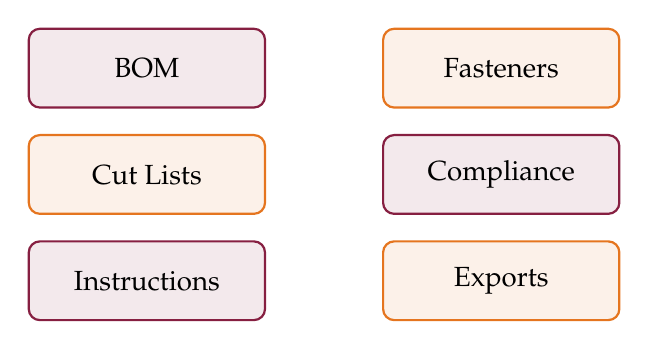
\begin{tikzpicture}[scale=0.9]
\node[draw=vtmaroon, thick, rounded corners, minimum width=3cm, minimum height=1cm, fill=vtmaroon!10] at (0,2) {BOM};
\node[draw=vtorange, thick, rounded corners, minimum width=3cm, minimum height=1cm, fill=vtorange!10] at (0,0.5) {Cut Lists};
\node[draw=vtmaroon, thick, rounded corners, minimum width=3cm, minimum height=1cm, fill=vtmaroon!10] at (0,-1) {Instructions};
\node[draw=vtorange, thick, rounded corners, minimum width=3cm, minimum height=1cm, fill=vtorange!10] at (5,2) {Fasteners};
\node[draw=vtmaroon, thick, rounded corners, minimum width=3cm, minimum height=1cm, fill=vtmaroon!10] at (5,0.5) {Compliance};
\node[draw=vtorange, thick, rounded corners, minimum width=3cm, minimum height=1cm, fill=vtorange!10] at (5,-1) {Exports};
\end{tikzpicture}

\vspace{2em}
{\large Every line item fully traceable}
\end{frame}

\begin{frame}{}
\centering
\vspace{3em}
{\LARGE \textbf{Provenance}}

\vspace{2em}
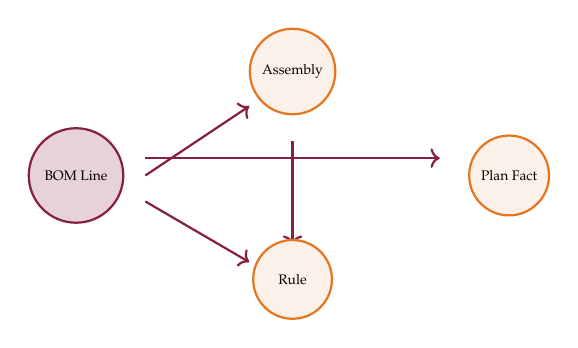
\begin{tikzpicture}[scale=1.1]
\node[circle, draw=vtmaroon, thick, minimum size=1.2cm, fill=vtmaroon!20, font=\tiny] at (0,0) {BOM Line};
\draw[->, thick, vtmaroon] (0.8,0) -- (2,0.8);
\node[circle, draw=vtorange, thick, minimum size=1cm, fill=vtorange!10, font=\tiny] at (2.5,1.2) {Assembly};
\draw[->, thick, vtmaroon] (2.5,0.4) -- (2.5,-0.8);
\node[circle, draw=vtorange, thick, minimum size=1cm, fill=vtorange!10, font=\tiny] at (2.5,-1.2) {Rule};
\draw[->, thick, vtmaroon] (0.8,-0.3) -- (2,-1);
\node[circle, draw=vtorange, thick, minimum size=1cm, fill=vtorange!10, font=\tiny] at (5,0) {Plan Fact};
\draw[->, thick, vtmaroon] (0.8,0.2) -- (4.2,0.2);
\end{tikzpicture}

\vspace{3em}
{\large Full audit trail from plan to procurement}
\end{frame}

% =============================================================================
% SECTION 6: IMPLEMENTATION
% =============================================================================
\section{Implementation Roadmap}

\begin{frame}{Current Status}
\begin{table}
\centering
\begin{tabular}{lcc}
\toprule
\textbf{Component} & \textbf{Status} & \textbf{Phase} \\
\midrule
DXF/DWG/PDF Parsing & \textcolor{green!60!black}{Complete} & 1 \\
Wall Extraction & \textcolor{green!60!black}{Complete} & 1 \\
Stud/Plate Calculation & \textcolor{green!60!black}{Complete} & 1 \\
YOLOv8 Detection & \textcolor{orange}{Partial} & 2 \\
Web Interface (React) & \textcolor{green!60!black}{Complete} & 1 \\
Docker Infrastructure & \textcolor{green!60!black}{Complete} & 1 \\
\midrule
Knowledge Graph & \textcolor{blue}{\textbf{New}} & 1--2 \\
Agent Orchestration & \textcolor{blue}{\textbf{New}} & 2 \\
Cut Optimization & \textcolor{blue}{\textbf{New}} & 2 \\
Code Compliance & \textcolor{blue}{\textbf{New}} & 3 \\
\bottomrule
\end{tabular}
\end{table}
\end{frame}

\begin{frame}{Phased Development}
\begin{description}
    \item[Phase 1] \textbf{KG Foundation} (4--6 weeks)
    \begin{itemize}
        \item Neo4j ontology, baseline rules, provenance tracking
    \end{itemize}

    \item[Phase 2] \textbf{Assembly Reasoning + Cut Optimization} (6--10 weeks)
    \begin{itemize}
        \item Component inference agent, OR-Tools integration
    \end{itemize}

    \item[Phase 3] \textbf{Code/Regulation Layer} (6--10 weeks)
    \begin{itemize}
        \item IRC/IBC modeling, compliance agent, citations
    \end{itemize}

    \item[Phase 4] \textbf{Feedback Loop} (Ongoing)
    \begin{itemize}
        \item Capture overrides, learn from outcomes
    \end{itemize}
\end{description}
\end{frame}

% =============================================================================
% SECTION 7: BUSINESS CASE
% =============================================================================
\section{Business Case}

\begin{frame}{}
\centering
\vspace{1em}
{\LARGE \textbf{Impact}}

\vspace{2em}
\begin{columns}
\column{0.5\textwidth}
\centering
{\Huge \textcolor{vtorange}{\textbf{70--80\%}}}

\vspace{0.5em}
{\large time saved}

\vspace{2em}
{\Huge \textcolor{vtmaroon}{\textbf{95\%+}}}

\vspace{0.5em}
{\large accuracy}

\column{0.5\textwidth}
\centering
{\Huge \textcolor{vtorange}{\textbf{<5\%}}}

\vspace{0.5em}
{\large waste}

\vspace{2em}
{\Huge \textcolor{vtmaroon}{\textbf{3--5×}}}

\vspace{0.5em}
{\large throughput}
\end{columns}
\end{frame}

\begin{frame}{}
\centering
\vspace{2em}
{\LARGE \textbf{ROI}}

\vspace{1em}
{\large Mid-size contractor (50 projects/year)}

\vspace{2em}
{\Huge \textcolor{vtorange}{\textbf{\$175K--\$250K}}}

\vspace{1em}
{\large annual benefit}

\vspace{3em}
{\Large Payback: \textcolor{vtmaroon}{\textbf{<6 months}}}
\end{frame}

% =============================================================================
% SECTION 8: CONCLUSION
% =============================================================================
\section{Conclusion}

\begin{frame}{}
\centering
\vspace{2em}
{\LARGE \textbf{Why Construction.AI?}}

\vspace{2em}
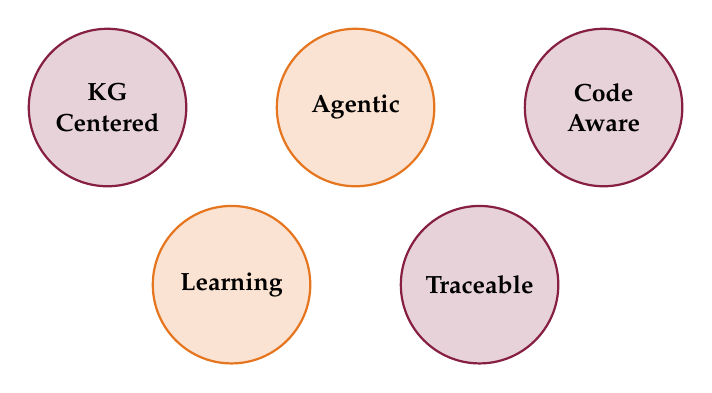
\begin{tikzpicture}[scale=0.9]
\node[draw=vtmaroon, thick, circle, minimum size=2cm, fill=vtmaroon!20, font=\small\bfseries, align=center] at (0,0) {KG\\Centered};
\node[draw=vtorange, thick, circle, minimum size=2cm, fill=vtorange!20, font=\small\bfseries, align=center] at (3.5,0) {Agentic};
\node[draw=vtmaroon, thick, circle, minimum size=2cm, fill=vtmaroon!20, font=\small\bfseries, align=center] at (7,0) {Code\\Aware};
\node[draw=vtorange, thick, circle, minimum size=2cm, fill=vtorange!20, font=\small\bfseries, align=center] at (1.75,-2.5) {Learning};
\node[draw=vtmaroon, thick, circle, minimum size=2cm, fill=vtmaroon!20, font=\small\bfseries, align=center] at (5.25,-2.5) {Traceable};
\end{tikzpicture}

\vspace{2em}
{\large Plan to procurement in \textcolor{vtorange}{\textbf{minutes}}}
\end{frame}

\begin{frame}{}
\centering
\vspace{4em}
{\Huge \textbf{Questions?}}

\vspace{4em}
{\large Jason Cusati}

{\small Virginia Tech}
\end{frame}

% =============================================================================
% BACKUP SLIDES
% =============================================================================
\appendix

\begin{frame}{Backup: KG Entity Schema}
\small
\begin{itemize}
    \item \textbf{Project} $\xrightarrow{\textit{hasSheet}}$ \textbf{PlanSheet}
    \item \textbf{PlanSheet} $\xrightarrow{\textit{mentions}}$ \textbf{PlanFact}
    \item \textbf{PlanFact} $\xrightarrow{\textit{instantiates}}$ \textbf{AssemblyIntent}
    \item \textbf{AssemblyIntent} $\xrightarrow{\textit{composedOf}}$ \textbf{Component}
    \item \textbf{Component} $\xrightarrow{\textit{builtFrom}}$ \textbf{StockItem}
    \item \textbf{StockItem} $\xrightarrow{\textit{cutInto}}$ \textbf{CutPiece}
    \item \textbf{Component} $\xrightarrow{\textit{requiresFastener}}$ \textbf{FastenerRule}
    \item \textbf{Component} $\xrightarrow{\textit{constrainedBy}}$ \textbf{CodeRule}
\end{itemize}
\end{frame}

\begin{frame}[fragile]{Backup: Sample JSON Output}
\tiny
\begin{verbatim}
{
  "project": "9557 Barnes Road",
  "assemblies": [{
    "type": "header_assembly",
    "opening": "Front Door",
    "components": [{
      "type": "header", "spec": "(2) 2x10",
      "length_in": 42, "stock_length": 144
    }],
    "fasteners": [{"type": "16d common", "qty": 24}],
    "code_ref": "IRC R602.7"
  }]
}
\end{verbatim}
\end{frame}

\end{document}
